\providecommand{\Fun}{\operatorname{Fun}}
\providecommand{\Cat}{\mathcal{C}at}
\providecommand{\sSet}{s\mathcal{S}et}
\providecommand{\QCat}{\mathcal{Q}\mathcal{C}at}
\providecommand{\CSS}{\mathcal{CSS}}
\providecommand{\rvEqArrow}{\mathrel{\stackrel{\sim}{\Rightarrow}}}
\providecommand{\rvTfibArrow}{\mathrel{\stackrel{\sim}{\twoheadrightarrow}}}
\section{\trInfinityCosmos}\label{sec:infinity-cosmos}

在 1.1 节中，我们给出了关于\trQuasiCategory{}若干基本事实的「分析的」证明。
\trQuasiCategory{}的范畴论固然可以按类似的风格发展，
但我们的目标毋宁是发展无穷维\trCategory{}的「综合的」理论，
使我们的结果能够同时适用于许多模型。为达此目的，
我们的策略不是去公理化无穷维\trCategory{}\emph{究竟是什么}，
而是去公理化它们所\emph{栖居}的范畴的「宇宙」。

\trInfinityCosmos{}的定义汲取了 1.1 节中引进的\trQuasiCategory{}\trCategory{}连同%
\trIsofibration{}、\trEquivalence{}与\trTrivialFibration{}的种种性质。%
\footnote{撇开隐喻性的典故不谈，我们的\trInfinityCosmos{}与
Street 的\trFibration{}式宇宙 \cite{bib117} 相类似。}
首先，\trQuasiCategory{}的\trCategory{}\emph{富集}于\trSimplicialSet{}的\trCategory{}之上——
从 $A$ 到 $B$ 的态射之集与\trSimplicialSet $B^A$ 的顶点之集相重合——
而且这些 hom 空间都是\trQuasiCategory{}。
其次，某些可以在\trQuasiCategory{}的非富集底范畴中定义的\trLimit{}构造
相对这种单纯富集满足泛性质，而且通常的集合\trIsomorphism{}可以扩充为\trSimplicialSet{}的\trIsomorphism{}。
最后，\trIsofibration{}、\trEquivalence{}与\trTrivialFibration{}满足一些
从抽象\trHomotopy{}论看来颇为熟悉的性质，
从而构成 Brown \cite{bib23} 意义下的\emph{\trFibration{}对象\trCategory}（见附录 C.1）。
特别地，在图表中使用\trIsofibration{}保证了它们的严格\trLimit{}是\trEquivalence{}不变的，
因此我们既能利用「到\trIsomorphism{}为止」的泛性质与这些构造的严格\trFunctor{}性，
又仍然在「\trHomotopy{}式地」工作。

正如\cref{dig:source-cosmoi-nature}中所解释的，有许多无穷维\trCategory{}的模型：
对其中的每一者，「\trInfinityCategory」（我们如此称呼它们）连同其间的「∞-\trFunctor」
所构成的\trCategory{}富集于\trQuasiCategory{}之上，
并且容许满足类似性质的\trIsofibration{}、\trEquivalence{}与\trTrivialFibration{}类。
这促成了如下的公理化。

\begin{definition}[\trInfinityCosmos]\label{def:infinity-cosmos}
一个\textbf{\trInfinityCosmos} $\mathcal{K}$
是一个富集于\trQuasiCategory{}之上的\trCategory{}，%
\footnote{这即是说 $\mathcal{K}$ 是一个\trSimpliciallyEnrichedCategory{}（见\cref{dig:simplicial-categories}），
其 hom 空间都是\trQuasiCategory{}。}
特别地，这意味着
\begin{itemize}
\item 它的态射 $f\colon A\to B$ 定义了某个\trQuasiCategory{}的顶点，
  该\trQuasiCategory{}记作 $\Fun(A,B)$，
  称为一个\textbf{\trFunctorSpace}（functor space），
\end{itemize}
而 $\mathcal{K}$ 还配备有指定的一类映射，
我们称之为\textbf{\trIsofibration{}}并记作「$\twoheadrightarrow$」，
满足以下两条公理：
\begin{enumerate}[label=(\roman*)]
\item （完备性）这个\trQuasiCategory\trEnrichedCategory $\mathcal{K}$ 拥有\trTerminal{}、小积、
  \trIsofibration{}的\trPullback{}、\trIsofibration{}的可数塔的\trLimit{}、
  以及与\trSimplicialSet{}的\trCotensor{}，
  这些\trLimit{}概念中的每一个都满足相对\trSimplicialSet{}富集的泛性质。%
  \footnote{我们在\cref{dig:simplicially-enriched-limits}中详述这些单纯富集的\trLimit{}。}
\item （\trIsofibration）\trIsofibration{}包含所有\trIsomorphism
  以及余域为\trTerminal{}的任何映射；
  在复合、积、\trPullback{}、取塔的逆\trLimit{}、
  以及与\trSimplicialSet{}的\trMonomorphism{}作 Leibniz \trCotensor{}下封闭；
  并且具有如下性质：若 $f\colon A\twoheadrightarrow B$
  是\trIsofibration{}且 $X$ 是任意对象，
  则 $\Fun(X,A)\twoheadrightarrow\Fun(X,B)$
  是\trQuasiCategory{}的\trIsofibration{}。
\end{enumerate}
\end{definition}

为便于引用，我们把 (i) 中列举的那些\trIsofibration{}图表的
单纯富集\trLimit{}统称为\textbf{\trCosmologicalLimitNotions}
（cosmological limit notions）。

\begin{definition}\label{def:equivalence-trivial-fibration}
在一个\trInfinityCosmos{}$\mathcal{K}$ 中，态射 $f\colon A\to B$ 是
\begin{itemize}
\item 一个\textbf{\trEquivalence}，当且仅当诱导映射
  $f_\ast\colon\Fun(X,A)\rvEqArrow\Fun(X,B)$
  在\trFunctorSpace{}上对一切 $X\in\mathcal{K}$
  是\trQuasiCategory{}的\trEquivalence{}，
\item 一个\textbf{\trTrivialFibration}，当且仅当 $f$
  既是\trIsofibration{}又是\trEquivalence{}。
\end{itemize}
这两个类分别记作「$\rvEqArrow$」与「$\rvTfibArrow$」。
\end{definition}

简而言之，或许可以说一个\trInfinityCosmos{}%
是一个「\trQuasiCategory{}富集的\trFibration{}对象\trCategory」
（见定义 C.1.1 与例 C.1.3）。

\begin{convention}[\trInfinityCategory{}，作为技术术语]\label{conv:infinity-category}
从此以后，我们重新把\textbf{\trInfinityCategory{}}设定为一个技术性术语，
指称任意周围\trInfinityCosmos{}中的对象。
类似地，我们用术语\textbf{∞-\trFunctor}——或者更常见地，其省略形式「\textbf{\trFunctor{}}」——
来指称\trInfinityCosmos{}中的态射 $f\colon A\to B$。
这也解释了为什么我们把\trInfinityCosmos{}中
两个\trInfinityCategory{}之间的\trQuasiCategory{} $\Fun(A,B)$
称为「\trFunctorSpace」：它的顶点正是从 $A$ 到 $B$ 的（∞-）\trFunctor{}。
\end{convention}

\begin{digression}[\trSimplicialCategory{}，附录 A.2]\label{dig:simplicial-categories}
一个\textbf{\trSimplicialCategory}（simplicial category）$\mathcal{A}$
由一些\trCategory{} $\mathcal{A}_n$ 给出：
它们带有共同的对象集，其箭头称为 $n$\textbf{-箭头}（$n$-arrows），
并且装配成一个由对象上恒等的\trFunctor{}构成的图表
$\boldsymbol{\Delta}^{op}\to\Cat$
\begin{rveq}\label{eq:simplicial-category-diagram}
\begin{tikzpicture}[xscale=0.95,yscale=1]
\node (A3) at (0,0) {$\cdots\,\mathcal{A}_3$};
\node (A2) at (4.1,0) {$\mathcal{A}_2$};
\node (A1) at (8.2,0) {$\mathcal{A}_1$};
\node (A0) at (11.9,0) {$\mathcal{A}_0$};
\node at (13.6,0) {$\coloneqq\mathcal{A}$};
\draw[->] (1.1,1.5) -- (3.1,1.5) node[midway,above]{$\scriptstyle\delta^3$};
\draw[->] (3.1,1.0) -- (1.1,1.0) node[midway,above]{$\scriptstyle\sigma^2$};
\draw[->] (1.1,0.5) -- (3.1,0.5) node[midway,above]{$\scriptstyle\delta^2$};
\draw[->] (3.1,0) -- (1.1,0) node[midway,above]{$\scriptstyle\sigma^1$};
\draw[->] (1.1,-0.5) -- (3.1,-0.5) node[midway,above]{$\scriptstyle\delta^1$};
\draw[->] (3.1,-1.0) -- (1.1,-1.0) node[midway,above]{$\scriptstyle\sigma^0$};
\draw[->] (1.1,-1.5) -- (3.1,-1.5) node[midway,above]{$\scriptstyle\delta^0$};
\draw[->] (5.2,1.0) -- (7.2,1.0) node[midway,above]{$\scriptstyle\delta^2$};
\draw[->] (7.2,0.5) -- (5.2,0.5) node[midway,above]{$\scriptstyle\sigma^1$};
\draw[->] (5.2,0) -- (7.2,0) node[midway,above]{$\scriptstyle\delta^1$};
\draw[->] (7.2,-0.5) -- (5.2,-0.5) node[midway,above]{$\scriptstyle\sigma^0$};
\draw[->] (5.2,-1.0) -- (7.2,-1.0) node[midway,above]{$\scriptstyle\delta^0$};
\draw[->] (9.3,0.5) -- (11.3,0.5) node[midway,above]{$\scriptstyle\delta^1$};
\draw[->] (11.3,0) -- (9.3,0) node[midway,above]{$\scriptstyle\sigma^0$};
\draw[->] (9.3,-0.5) -- (11.3,-0.5) node[midway,above]{$\scriptstyle\delta^0$};
\end{tikzpicture}
\end{rveq}
$0$-箭头的\trCategory{} $\mathcal{A}_0$ 是\trSimplicialCategory $\mathcal{A}$ 的
\textbf{底范畴}（underlying category），
它遗忘掉高维的单纯结构。

\trSimplicialCategory{}的数据也可以\trEquivalence{}地用一个\textbf{\trSimpliciallyEnrichedCategory}
（simplicially enriched category）来编码：
它有一个对象集，并对每一对有序对象配有态射的\trSimplicialSet $\mathcal{A}(x,y)$：
$\mathcal{A}_n$ 中从 $x$ 到 $y$ 的 $n$-箭头对应于
$\mathcal{A}(x,y)$ 中的一个 $n$-单纯形（见\cref{ex:simplicial-versus-enriched}）。
每个自同态 hom 空间都含有一个特别的恒等 $0$-箭头
（其退化像定义相应的恒等 $n$-箭头），
并且要求复合定义一个\trSimplicialMap
\begin{equation*}
\mathcal{A}(y,z)\times\mathcal{A}(x,y)
\xrightarrow{\ \circ\ }\mathcal{A}(x,z)
\end{equation*}
这一单独的映射同时编码了每个\trCategory{} $\mathcal{A}_n$ 中的复合
以及图表 \eqref{eq:simplicial-category-diagram} 的\trFunctor{}性。
复合被要求是结合且幺一的，
其含义由\trSimplicialSet{}的如下交换图表表达
\begin{equation*}
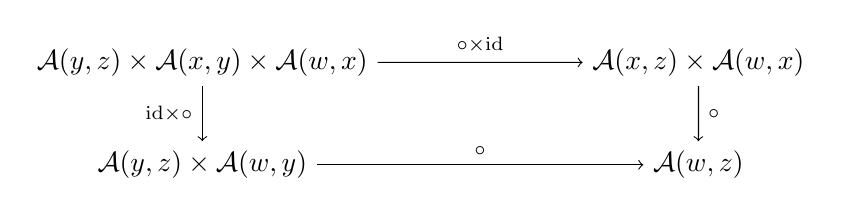
\begin{tikzpicture}[xscale=1.5,yscale=1.3]
\node (TL) at (0,1) {$\mathcal{A}(y,z)\times\mathcal{A}(x,y)\times\mathcal{A}(w,x)$};
\node (TR) at (4.2,1) {$\mathcal{A}(x,z)\times\mathcal{A}(w,x)$};
\node (BL) at (0,0) {$\mathcal{A}(y,z)\times\mathcal{A}(w,y)$};
\node (BR) at (4.2,0) {$\mathcal{A}(w,z)$};
\draw[->] (TL) -- (TR) node[midway,above]{$\scriptstyle\circ\times\mathrm{id}$};
\draw[->] (TL) -- (BL) node[midway,left]{$\scriptstyle\mathrm{id}\times\circ$};
\draw[->] (TR) -- (BR) node[midway,right]{$\scriptstyle\circ$};
\draw[->] (BL) -- (BR) node[midway,above]{$\scriptstyle\circ$};
\end{tikzpicture}
\end{equation*}
\begin{equation*}
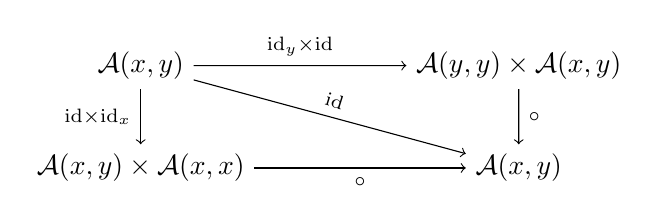
\begin{tikzpicture}[xscale=1.5,yscale=1.3]
\node (TL) at (0,1) {$\mathcal{A}(x,y)$};
\node (TR) at (3.2,1) {$\mathcal{A}(y,y)\times\mathcal{A}(x,y)$};
\node (BL) at (0,0) {$\mathcal{A}(x,y)\times\mathcal{A}(x,x)$};
\node (BR) at (3.2,0) {$\mathcal{A}(x,y)$};
\draw[->] (TL) -- (TR) node[midway,above]{$\scriptstyle\mathrm{id}_y\times\mathrm{id}$};
\draw[->] (TL) -- (BL) node[midway,left]{$\scriptstyle\mathrm{id}\times\mathrm{id}_x$};
\draw[->] (TL) -- (BR) node[midway,above,sloped]{$\scriptstyle\mathrm{id}$};
\draw[->] (TR) -- (BR) node[midway,right]{$\scriptstyle\circ$};
\draw[->] (BL) -- (BR) node[midway,below]{$\scriptstyle\circ$};
\end{tikzpicture}
\end{equation*}
由于这两种表述之间的\trEquivalence{}，
「\trSimplicialCategory」与「\trSimpliciallyEnrichedCategory」这两个术语通常被视为同义词。
\footnote{「$\Cat$ 中的单纯对象」一语保留给更一般却不那么常见的概念：
不必然由对象上恒等的\trFunctor{}构成的图表
$\boldsymbol{\Delta}^{op}\to\Cat$。}

特别地，\trInfinityCosmos{} $\mathcal{K}$ 的底范畴 $\mathcal{K}_0$
是这样的\trCategory{}：其对象是 $\mathcal{K}$ 中的\trInfinityCategory{}，
其态射是 $0$-箭头，即\trFunctorSpace{}中的顶点。
在下文将要出现的所有例子中，
这都复原出特定模型下\trInfinityCategory{}及其间\trFunctor{}的
所期望的\trCategory{}。
\end{digression}

\begin{digression}[\trSimpliciallyEnrichedLimit{}，附录 A.4–A.5]\label{dig:simplicially-enriched-limits}
设 $\mathcal{A}$ 为\trSimplicialCategory{}。对象 $A\in\mathcal{A}$
由\trSimplicialSet $U$ 作出的\textbf{\trCotensor}（cotensor）
由\trSimplicialSet{}的自然\trIsomorphism{}刻画
\begin{rveq}\label{eq:cotensor-universal}
\mathcal{A}(X,A^U)\cong\mathcal{A}(X,A)^U
\end{rveq}
假定这样的对象存在，
单纯\trCotensor{}便以唯一的方式定义一个双\trFunctor
\begin{equation*}
\begin{gathered}
\sSet^{op}\times\mathcal{A}\longrightarrow\mathcal{A}\\
(U,A)\longmapsto A^U
\end{gathered}
\end{equation*}
使得\trIsomorphism \eqref{eq:cotensor-universal} 在 $U$ 与 $A$ 上也自然。
\cref{def:infinity-cosmos}(i) 所假定的其余单纯\trLimit{}概念是\textbf{\trCone{}形的}（conical）——
这一术语用于通常的 1-范畴论\trLimit{}形状，
它们满足通常泛性质的一个富集类比（见定义 A.5.2）。
这样的\trLimit{}也定义底范畴中的\trLimit{}，但通常的泛性质被加强了。
把协变\trRepresentable{}\trFunctor
$\mathcal{A}(X,-)\colon\mathcal{A}_0\to\sSet$
用于 $\mathcal{A}_0$ 中的\trLimit{}\trCone
$(\lim_{j\in J}A_j\to A_j)_{j\in J}$，
我们得到一个自然比较映射
\begin{rveq}\label{eq:conical-comparison}
\mathcal{A}\Bigl(X,\lim_{j\in J}A_j\Bigr)
\longrightarrow\lim_{j\in J}\mathcal{A}(X,A_j).
\end{rveq}
我们说 $\lim_{j\in J}A_j$ 定义了一个\textbf{\trSimpliciallyEnrichedLimit}
（simplicially enriched limit），
当且仅当 \eqref{eq:conical-comparison}
对一切 $X\in\mathcal{A}$ 是\trSimplicialSet{}的\trIsomorphism{}。
\end{digression}

\trEnrichedCategory{}的一般理论在附录 A 中综述。

\begin{preview}[\trInfinityCosmos{}中的柔性加权\trLimit]\label{pv:flexible-weighted-limits}
\cref{def:infinity-cosmos}(i) 蕴含：任何\trInfinityCosmos{} $\mathcal{K}$
都容许所有\emph{柔性极限}（flexible limits）——
远更大的一类单纯富集的「加权」\trLimit
（见定义 6.2.1 与命题 6.2.8）。
\end{preview}

我们快速介绍三个最容易被吸收的\trInfinityCosmos{}例子，
把更精致的例子推迟到本节末尾。
其中第一个是原型性的\trInfinityCosmos{}。

\begin{proposition}[\trQuasiCategory{}的\trInfinityCosmos]\label{prop:cosmos-quasi-categories}
\trQuasiCategory{}的满子\trCategory $\QCat\subset\sSet$
定义一个\trInfinityCosmos{}，其中\trIsofibration{}、\trEquivalence{}与\trTrivialFibration{}%
恰与已具有这些名称的诸类相重合。
\end{proposition}
\begin{proof}
子\trCategory $\QCat\subset\sSet$ 的单纯富集继承自\trSimplicialSet{}的笛卡尔封闭\trCategory{}：
由命题 1.1.20，每当 $A$ 与 $B$ 是\trQuasiCategory{}， %
$\Fun(A,B):=B^A$ 仍是\trQuasiCategory{}。
\cref{def:infinity-cosmos}(i) 中假定的宇宙论\trLimit{}存在于周围的\trSimplicialSet\trCategory{}中。%
\footnote{任何预层\trCategory{}都是笛卡尔封闭、完备且余完备的——
Bénabou 意义下的一个「宇宙」。}
例如，单纯\trCotensor \eqref{eq:cotensor-universal} 的定义性泛性质
由\trSimplicialSet{}的指数满足。此外，由于\trSimplicialSet{}的\trCategory{}是\trCartesianClosed{}，
每个\trCone{}形\trLimit{}都在\cref{dig:simplicially-enriched-limits}所讨论的意义下单纯富集
（见\cref{ex:conical-products-qcat}与命题 A.5.4）。

我们现在论证\trQuasiCategory{}的满子\trCategory{}继承所有这些\trLimit{}概念，
同时建立\trIsofibration{}在这些\trLimit{}的构造下的稳定性。
事实上，后一性质有助于证明前一性质。
为看到这一点，注意\trSimplicialSet{}是\trQuasiCategory{}，当且仅当
从它到点的映射是\trIsofibration{}。
更一般地，若任何\trIsofibration{}的余域是\trQuasiCategory{}，
则其定义域也必是。
于是，若\trQuasiCategory{}图表上的\trLimit{}\trCone{}中只要有映射是\trIsofibration{}，
便可推出该\trLimit{}本身是\trQuasiCategory{}。

由于\trIsofibration{}由右提升性质刻画，
引理 C.2.3 蕴含\trIsofibration{}包含所有\trIsomorphism{}，
并且在复合、积、\trPullback{}与取塔的逆\trLimit{}下封闭。
特别地，\trQuasiCategory{}的满子\trCategory{}拥有这些\trLimit{}。
这就验证了 \cref{def:infinity-cosmos}(i) 与 (ii) 的全部公理，
除了最后两条：Leibniz 封闭性与对取指数 $(-)^X$ 的封闭性。
这最后的封闭性质已在命题 1.1.20 中建立， %
而且事实上由练习 1.1.vii，前者涵盖后者。
这就完成了对\trInfinityCosmos{}公理的验证。

剩下要检查的是\trEquivalence{}与\trTrivialFibration
恰与 1.1.23 及 1.1.25 所定义的映射重合。 %
由命题 1.1.28，后一重合由前一重合推出， %
故只剩下证明 1.1.23 的\trEquivalence{}与 %
\textbf{可表示地定义的\trEquivalence}（representably defined equivalences）
重合：即那些使 $A^X\to B^X$ 成为定义 1.1.23 意义下\trQuasiCategory{}的%
\trEquivalence{}的%
\trQuasiCategory{}映射 $f\colon A\to B$。
取 $X=\Delta[0]$，立即可见可表示地定义的\trEquivalence{}是\trEquivalence{}，
而逆命题成立，因为指数 $(-)^X$
保持定义单纯\trHomotopy{}的数据。
\end{proof}

另外两个例子符合同一范式：
二者都作为\trQuasiCategory{}的\trInfinityCosmos{}的满子\trCategory{}出现，
并从这个包含继承其\trInfinityCosmos{}结构（见引理 6.1.4）。
但描述所得到的\trInfinityCosmos{}结构本身也富有教益，
而且归根结底工作量更小。

\begin{proposition}[\trCategory{}的\trInfinityCosmos]\label{prop:cosmos-categories}
1-\trCategory{}的\trCategory{} $\Cat$
定义一个\trInfinityCosmos{}，其\trIsofibration{}恰是
\textbf{\trIsofibration}：即满足下图所示右提升性质的\trFunctor
\begin{center}
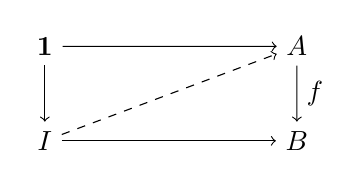
\begin{tikzpicture}[xscale=1.6,yscale=1.2]
\node (TL) at (0,1) {$\mathbf{1}$};
\node (TR) at (2,1) {$A$};
\node (BL) at (0,0) {$\mathbb{I}$};
\node (BR) at (2,0) {$B$};
\draw[->] (TL) -- (TR);
\draw[->] (TL) -- (BL);
\draw[->] (BL) -- (BR);
\draw[->] (TR) -- (BR) node[midway,right]{$f$};
\draw[dashed,->] (BL) -- (TR);
\end{tikzpicture}
\end{center}
\trEquivalence{}恰是\trCategory{}的\trEquivalence{}，而\trTrivialFibration{}恰是
\textbf{满射\trEquivalence}（surjective equivalences）：
在对象上也为满射的\trCategory\trEquivalence{}。
\end{proposition}
\begin{proof}
众所周知，\trCategory{}的 2-\trCategory{}作为 $\Cat$-富集的\trCategory{}是完备的
（其实也余完备）（见定义 A.6.17 或文献 \cite{bib67}）。
把\trNerve\trFunctor{}用于 hom-\trCategory{}，
\trCategory{}的这个\trEnrichedCategory{}便成为\trQuasiCategory\trEnrichedCategory{}（见附录 A.7）。
由于\trNerve\trFunctor{}是右\trAdjunction{}，
这些 2-范畴论的\trLimit{}在形式上变成单纯富集\trLimit{}。
特别地，如命题 A.7.8 所规定的，
\trCategory{} $A$ 由\trSimplicialSet $U$ 作出的\trCotensor
定义为\trFunctor{}\trCategory $A^{hU}$。
这就完成了公理 (i) 的验证。

由于\trIsofibration{}的类由右提升性质刻画，
引理 C.2.3 蕴含\trIsofibration{}对 \cref{def:infinity-cosmos}(ii)
除最后两条之外的所有\trLimit{}构造封闭；
而由练习 1.1.vii，Leibniz 封闭性涵盖对取指数的封闭性。

要验证\trCategory{}的\trIsofibration{} $f\colon A\twoheadrightarrow B$
在与\trSimplicialSet{}的\trMonomorphism $i\colon U\hookrightarrow V$
作 Leibniz \trCotensor{}下的稳定性，
我们必须求解左下的\trLifting{}问题
\begin{equation*}
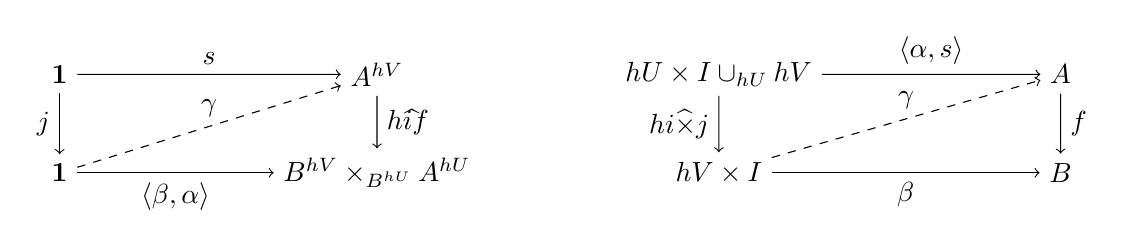
\begin{tikzpicture}[xscale=1.55,yscale=1.25]
\node (TL) at (0,1) {$\mathbf{1}$};
\node (TR) at (2.6,1) {$A^{hV}$};
\node (BL) at (0,0) {$\mathbf{1}$};
\node (BR) at (2.6,0) {$B^{hV}\times_{B^{hU}}A^{hU}$};
\draw[->] (TL) -- (TR) node[midway,above]{$s$};
\draw[->] (TL) -- (BL) node[midway,left]{$j$};
\draw[->] (BL) -- (BR) node[midway,below]{$\langle\beta,\alpha\rangle$};
\draw[->] (TR) -- (BR) node[midway,right]{$hi\widehat{\pitchfork}f$};
\draw[dashed,->] (BL) -- (TR) node[midway,above]{$\gamma$};
\node at (4.15,0.5) {$\leftrightsquigarrow$};
\node (rTL) at (5.4,1) {$hU\times\mathbb{I}\cup_{hU}hV$};
\node (rTR) at (8.2,1) {$A$};
\node (rBL) at (5.4,0) {$hV\times\mathbb{I}$};
\node (rBR) at (8.2,0) {$B$};
\draw[->] (rTL) -- (rTR) node[midway,above]{$\langle\alpha,s\rangle$};
\draw[->] (rTL) -- (rBL) node[midway,left]{$hi\widehat{\times}j$};
\draw[->] (rBL) -- (rBR) node[midway,below]{$\beta$};
\draw[->] (rTR) -- (rBR) node[midway,right]{$f$};
\draw[dashed,->] (rBL) -- (rTR) node[midway,above]{$\gamma$};
\end{tikzpicture}
\end{equation*}
它转置为右上的\trLifting{}问题，而后者可以手工求解。
这里映射 $\beta$ 定义了 $fs\colon hV\to B$
与另一个\trFunctor{}之间的自然\trIsomorphism{}。
我们的任务是把它\trLifting{}为从 $s$ 到另一\trFunctor{}的自然\trIsomorphism $\gamma$，
使 $\gamma$ 沿 $hi\colon hU\to hV$ 延拓自然\trIsomorphism $\alpha$。
注意\trFunctor{} $hi$ 未必是包含，
但它在对象上单射，这就够了。

我们分情形定义 $\gamma$ 的分量。
若对象 $v\in hV$ 等于某个 $u\in hU$ 的像 $i(u)$，
则定义 $\gamma_{i(u)}:=\alpha_u$；
否则，利用 $f$ 是\trIsofibration{}这一事实，
把\trIsomorphism $\beta_v$ \trLifting{}为 $A$ 中以 $s(v)$ 为定义域的\trIsomorphism{}，从而定义 $\gamma_v$。
映射 $\gamma\colon hV\times\mathbb{I}\to A$ 的数据
还蕴含指定作为自然\trIsomorphism $\gamma$ 之余域的\trFunctor{} $hV\to A$。
在对象上，该\trFunctor{}由 $v\mapsto\mathrm{cod}(\gamma_v)$ 给出；
在态射上，它以唯一的方式定义，使得 $\gamma$ 成为\trNaturalTransformation
\begin{equation*}
(k\colon v\to v^{\prime})\mapsto
\gamma_{v^{\prime}}\circ s(k)\circ\gamma_v^{-1}.
\end{equation*}
这就完成了 $\Cat$ 定义一个\trInfinityCosmos{}的证明。
由于\trFunctor{}\trCategory{}（如 $A^{\mathbb{I}}$）的\trNerve
\trIsomorphism{}于其\trNerve{}之间的指数，
\trCategory{}的\trEquivalence{}恰与定义 1.1.23 的\trEquivalence{}重合。 %
于是\trCategory{}的\trInfinityCosmos{}中的\trEquivalence{}%
恰与\trCategory{}的\trEquivalence{}重合，
而由于满射\trEquivalence{}是\trEquivalence{}与\trIsofibration{}之交，
证明完毕。
\end{proof}

\begin{proposition}[\trKanComplex{}的\trInfinityCosmos]\label{prop:cosmos-kan-complexes}
\trKanComplex{}的\trCategory{} $\mathcal{K}an$
定义一个\trInfinityCosmos{}，其\trIsofibration{}恰是
\textbf{\trKanFibration}（Kan fibrations）：
即对所有 $n\geq 1$ 与 $0\leq k\leq n$
对一切\trHorn{}包含 $\Lambda^k[n]\hookrightarrow\Delta[n]$ 可\trLifting{}的映射。
\end{proposition}
其证明沿引理 6.1.4 的路线进行。
我们证明\trKanComplex{}的子\trCategory
通过从\trQuasiCategory{}的\trInfinityCosmos{}限制结构
而继承一个\trInfinityCosmos{}结构。
\begin{proof}
由命题 1.1.18，\trKanComplex{}之间的\trIsofibration{}是\trKanFibration{}。 %
反之，由于\trHomotopyCoherentIsomorphism $\mathbb{I}$
可以从点 $\mathbf{1}$ 出发、通过对外\trHorn{}逐个贴上填充物而构造出来，
所有\trKanFibration{}都定义\trIsofibration{}。
这表明\trKanComplex{}之间\trIsofibration{}与\trKanFibration{}重合。
于是，为证明\trKanComplex{}的\trCategory{}通过从\trQuasiCategory{}的%
\trInfinityCosmos{}限制而继承\trInfinityCosmos{}结构，
我们只需验证满子\trCategory $\mathcal{K}an\hookrightarrow\QCat$
对 \cref{def:infinity-cosmos}(i) 的所有\trLimit{}构造封闭。
对\trCone{}形\trLimit{}，论证与\cref{prop:cosmos-quasi-categories}之证明所给的论证互为镜像；
而对\trCotensor{}的封闭性则是推论 D.3.11 的推论， %
后者蕴含\trKanComplex{}在\trSimplicialSet{}的\trCategory{}中也定义一个\trExponentialIdeal{}。
其余公理，即 \cref{def:infinity-cosmos}(ii)，则从\cref{prop:cosmos-quasi-categories}中
对\trQuasiCategory{}建立的类似性质继承而来。
\end{proof}

我们对熟悉 Quillen \trModelCategory——抽象\trHomotopy{}论的一个流行框架——的读者，
提及一个自然界中\trInfinityCosmos{}的共同来源以建立直观；
同时也让新来者放心：在证明这些结果的附录 E 之外，
并不需要\trModelCategory{}。

\begin{digression}[自然界中\trInfinityCosmos{}的一个来源]\label{dig:source-cosmoi-nature}
如附录 E.1 中所解释的，
\trModelCategory{}的某些易于描述的性质蕴含：
\trFibration{}对象的满子\trCategory{}定义一个\trInfinityCosmos{}，
其\trIsofibration{}、\trEquivalence{}与\trTrivialFibration
恰是\trFibration{}对象之间的\trFibration{}、弱\trEquivalence{}与\trTrivialFibration{}。
也就是说，任何\trModelCategory{}，
只要它如此富集于\trSimplicialSet{}的 Joyal \trModelStructure{}之上、
且其中所有\trFibration{}对象都是余\trFibration{}的，
就呈现一个\trInfinityCosmos{}（见命题 E.1.1）。
这种对\trQuasiCategory{}的模型范畴论式富集
可以在\trModelCategory{}为笛卡尔封闭、
且配备有到\trSimplicialSet{}的 Joyal \trModelStructure{}的右 Quillen \trAdjunction{}、
其左\trAdjunction{}保持有限积时定义（见推论 E.1.4）。
此时，右\trAdjunction{}成为底\trQuasiCategory\trFunctor
（见命题 1.3.4(ii)）， %
而且如此产生的诸\trInfinityCosmos{}是\trCartesianClosed
（见\cref{def:cartesian-closed-cosmoi}）。
\cref{exa:cosmoi-models}中列出的诸\trInfinityCosmos{}全都以这种方式产生。
\end{digression}

下列结果是定义 1.2.1 的公理的推论。
首先，观察到\trTrivialFibration
享有与\trIsofibration{}相同的稳定性性质。

\begin{lemma}[\trTrivialFibration{}的稳定性]\label{lem:trivial-fibration-stability}
\trInfinityCosmos{}中的\trTrivialFibration{}定义一个包含所有\trIsomorphism{}的子\trCategory{}，
并且在积、\trPullback{}与取塔的逆\trLimit{}下稳定。
此外，任何\trTrivialFibration{}与\trSimplicialSet{}\trMonomorphism{}的 Leibniz \trCotensor{}是\trTrivialFibration{}， %
\trIsofibration{}与由内\trHorn{}包含及映射
$\mathbf{1}\hookrightarrow\mathbb{I}$
\trCell{}式生成的类中映射的 Leibniz \trCotensor{}亦然；
且若 $E\rvTfibArrow B$ 是\trTrivialFibration{}，
则 $\Fun(X,E)\rvTfibArrow\Fun(X,B)$ 亦然。
\end{lemma}
\begin{proof}
我们按相反的顺序证明这些陈述。
由 \cref{def:infinity-cosmos}(ii) 及\trInfinityCosmos{}中\trTrivialFibration{}的定义，我们知道：
若 $E\rvTfibArrow B$ 是\trTrivialFibration{}，
则 $\Fun(X,E)\rvTfibArrow\Fun(X,B)$
既是\trIsofibration{}又是\trEquivalence{}，
从而由命题 1.1.28 是\trTrivialFibration{}。 %
对其余构造的稳定性，
我们在每种情形都知道所涉映射是\trInfinityCosmos{}中的\trIsofibration{}；
剩下的只是证明这些映射也是\trEquivalence{}。
\trInfinityCosmos{}中的\trEquivalence{}%
被定义为被 $\Fun(X,-)$ 载为\trQuasiCategory{}之\trEquivalence{}的那些映射，
故只需验证\trQuasiCategory{}的\trTrivialFibration{}满足相应的稳定性性质。
对 Leibniz 稳定性性质，这已在命题 1.1.29 中建立，
而其余性质由引理 C.2.3 覆盖。
\end{proof}

由一个 Yoneda 式的论证，
定义 1.1.23 中\trQuasiCategory{}的\trInfinityCosmos{}的%
\trEquivalence{}的「\trHomotopyEquivalence」刻画，
可以扩充为任何\trInfinityCosmos{}中\trEquivalence{}的类似刻画：

\begin{lemma}[\trEquivalence{}是\trHomotopyEquivalence]\label{lem:equiv-homotopy-equivalences}
\trInfinityCosmos{} $\mathcal{K}$ 中\trInfinityCategory{}之间的
映射 $f\colon A\to B$ 是\trEquivalence{}，当且仅当
它扩充为「\trHomotopyEquivalence」的数据，
并以\trFreeLivingIsomorphism $\mathbb{I}$ 作为区间：
也就是说，若存在映射 $g\colon B\to A$
\begin{rveq}\label{eq:homotopy-equivalence-data}
\begin{tikzpicture}[xscale=1.35,yscale=1.05]
\node (lA) at (0,0) {$A$};
\node (tA) at (2.2,1.3) {$A$};
\node (Ai) at (2.2,0) {$A^{\mathbb{I}}$};
\node (bA) at (2.2,-1.3) {$A$};
\draw[double] (lA) -- (tA);
\draw[->] (Ai) -- (tA) node[midway,right]{$\mathrm{ev}_0$};
\draw[->] (lA) -- (Ai) node[midway,above]{$\alpha$};
\draw[->] (lA) -- (bA) node[midway,below]{$gf$};
\draw[->] (Ai) -- (bA) node[midway,right]{$\mathrm{ev}_1$};
\node at (4.1,0) {及};
\node (lB) at (6,0) {$B$};
\node (tB) at (8.2,1.3) {$B$};
\node (Bi) at (8.2,0) {$B^{\mathbb{I}}$};
\node (bB) at (8.2,-1.3) {$B$};
\draw[->] (lB) -- (tB) node[midway,above]{$fg$};
\draw[->] (Bi) -- (tB) node[midway,right]{$\mathrm{ev}_0$};
\draw[->] (lB) -- (Bi) node[midway,above]{$\beta$};
\draw[double] (lB) -- (bB);
\draw[->] (Bi) -- (bB) node[midway,right]{$\mathrm{ev}_1$};
\end{tikzpicture}
\end{rveq}
在\trInfinityCosmos{}之中。
\end{lemma}
\begin{proof}
按假设，若 $f\colon A\to B$ 定义\trInfinityCosmos{} $\mathcal{K}$
中的\trEquivalence{}，
则复合后诱导的映射 $f_\ast\colon\Fun(B,A)\rvEqArrow\Fun(B,B)$
是定义 1.1.23 意义下\trQuasiCategory{}的\trEquivalence{}。 %
在 $0$-箭头 $\mathrm{id}_B\in\Fun(B,B)$ 处
取值于逆\trEquivalence{} $\tilde{g}\colon\Fun(B,B)\rvEqArrow\Fun(B,A)$
与\trHomotopy $\tilde{\beta}\colon\Fun(B,B)\to\Fun(B,B)^{\mathbb{I}}$，
我们得到 $0$-箭头 $g\colon B\to A$，
连同从复合 $fg$ 到 $\mathrm{id}_B$
的\trIsomorphism $\beta\colon\mathbb{I}\to\Fun(B,B)$。
由\trCotensor \eqref{eq:cotensor-universal} 的定义性泛性质，
这一\trIsomorphism{}内部化而定义 $\mathcal{K}$ 中的映射
$\beta\colon B\to B^{\mathbb{I}}$，
即 \eqref{eq:homotopy-equivalence-data} 右侧所示者。

现在，$f$ 是\trEquivalence{}这一假设还提供%
\trQuasiCategory{}的\trEquivalence{} $f_\ast\colon\Fun(A,A)\rvEqArrow\Fun(A,B)$，
而映射 $\beta f\colon A\to B^{\mathbb{I}}$
表示 $\Fun(A,B)$ 中从 $fgf$ 到 $f$ 的\trIsomorphism{}。
由于 $f_\ast$ 是\trEquivalence{}，
我们从注 1.1.24 得出 $\mathrm{id}_A$ 与 $gf$
在\trQuasiCategory $\Fun(A,A)$ 中\trIsomorphism{}：
显式地，这样的\trIsomorphism{}可以这样定义——
取逆\trEquivalence{} $\tilde{h}\colon\Fun(A,B)\to\Fun(A,A)$，
并与从 $\mathrm{id}_{\Fun(A,A)}$ 到 $\tilde{h}f_\ast$
的\trIsomorphism $\tilde{\alpha}\colon\Fun(A,A)\to\Fun(A,A)^{\mathbb{I}}$
在 $\mathrm{id}_A$ 与 $gf\in\Fun(A,A)$ 处的分量作复合。
现在由推论 1.1.16，
这一\trIsomorphism{}由从 $\mathrm{id}_A$ 到 $gf$ 的映射
$\mathbb{I}\to\Fun(A,A)$ 表示，
后者内部化为 $\mathcal{K}$ 中的映射 $\alpha\colon A\to A^{\mathbb{I}}$，
即 \eqref{eq:homotopy-equivalence-data} 左侧所示者。

逆命题容易：
单纯\trCotensor{}构造与 $\Fun(X,-)$ 交换，
故\trHomotopyEquivalence \eqref{eq:homotopy-equivalence-data} 诱导
定义 1.1.23 意义下\trQuasiCategory{}的\trHomotopyEquivalence{}。 %
\end{proof}

\begin{lemma}\label{lem:equivalence-retracts-2-of-3}
\trInfinityCosmos{}中的\trEquivalence{}对收缩封闭，
并满足\textbf{\trTwoOfThreeProperty}（2-of-3 property）：
给定可复合的一对\trFunctor{}及其复合，
若其中任何两个是\trEquivalence{}，则第三个亦然。
\end{lemma}
由\trEquivalence{}的可表示定义与\trFunctor{}性，
\cref{lem:equivalence-retracts-2-of-3} 从\trQuasiCategory{}之间%
\trEquivalence{}的相应结果
（见练习 1.1.viii）容易推出。
但为完备起见，
我们不依赖这一基础情形而证明一般的宇宙论结果，
从而涵盖练习 1.1.viii。
\begin{proof}
设 $f\colon A\rvEqArrow B$ 是配有
\eqref{eq:homotopy-equivalence-data} 之数据的\trEquivalence{}，
并考虑收缩图表
\begin{center}
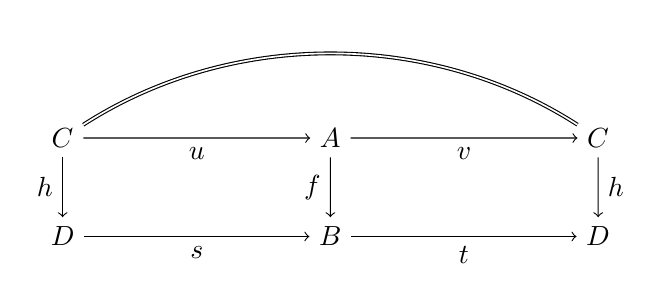
\begin{tikzpicture}[xscale=1.7,yscale=1.25]
\node (CL) at (0,1) {$C$};
\node (A) at (2,1) {$A$};
\node (CR) at (4,1) {$C$};
\node (DL) at (0,0) {$D$};
\node (B) at (2,0) {$B$};
\node (DR) at (4,0) {$D$};
\draw[double] (CL) to[out=40,in=140] (CR);
\draw[->] (CL) -- (A) node[midway,below]{$u$};
\draw[->] (A) -- (CR) node[midway,below]{$v$};
\draw[->] (CL) -- (DL) node[midway,left]{$h$};
\draw[->] (A) -- (B) node[midway,left]{$f$};
\draw[->] (CR) -- (DR) node[midway,right]{$h$};
\draw[->] (DL) -- (B) node[midway,below]{$s$};
\draw[->] (B) -- (DR) node[midway,below]{$t$};
\end{tikzpicture}
\end{center}
由\cref{lem:equiv-homotopy-equivalences}，要证 $h\colon C\to D$ 是\trEquivalence{}，
只需构造逆\trHomotopyEquivalence{}的数据。
为此定义 $k\colon D\to C$ 为复合 $vgs$，
然后从交换图表
\begin{center}
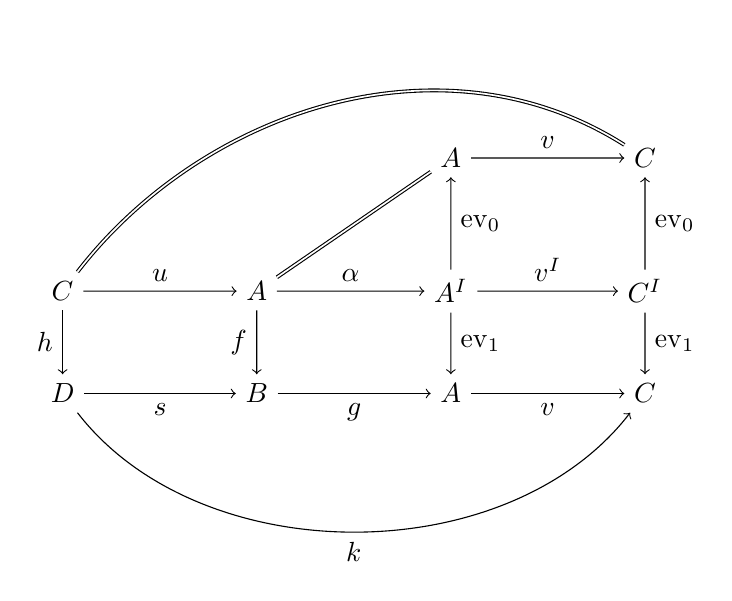
\begin{tikzpicture}[xscale=1.45,yscale=1.3]
\node (Cm) at (0,1) {$C$};
\node (A2) at (1.7,1) {$A$};
\node (Ai) at (3.4,1) {$A^{\mathbb{I}}$};
\node (Ci) at (5.1,1) {$C^{\mathbb{I}}$};
\node (At) at (3.4,2.3) {$A$};
\node (Ct) at (5.1,2.3) {$C$};
\node (D) at (0,0) {$D$};
\node (B) at (1.7,0) {$B$};
\node (Ab) at (3.4,0) {$A$};
\node (Cb) at (5.1,0) {$C$};
\draw[double] (Cm) to[out=55,in=145] (Ct);
\draw[->] (At) -- (Ct) node[midway,above]{$v$};
\draw[double] (A2) -- (At);
\draw[->] (Cm) -- (A2) node[midway,above]{$u$};
\draw[->] (A2) -- (Ai) node[midway,above]{$\alpha$};
\draw[->] (Ai) -- (Ci) node[midway,above]{$v^{\mathbb{I}}$};
\draw[->] (Ai) -- (At) node[midway,right]{$\mathrm{ev}_0$};
\draw[->] (Ci) -- (Ct) node[midway,right]{$\mathrm{ev}_0$};
\draw[->] (Ai) -- (Ab) node[midway,right]{$\mathrm{ev}_1$};
\draw[->] (Ci) -- (Cb) node[midway,right]{$\mathrm{ev}_1$};
\draw[->] (Cm) -- (D) node[midway,left]{$h$};
\draw[->] (A2) -- (B) node[midway,left]{$f$};
\draw[->] (D) -- (B) node[midway,below]{$s$};
\draw[->] (B) -- (Ab) node[midway,below]{$g$};
\draw[->] (Ab) -- (Cb) node[midway,below]{$v$};
\draw[->] (D) to[out=-55,in=-125] node[midway,below]{$k$} (Cb);
\end{tikzpicture}
\end{center}
\begin{center}
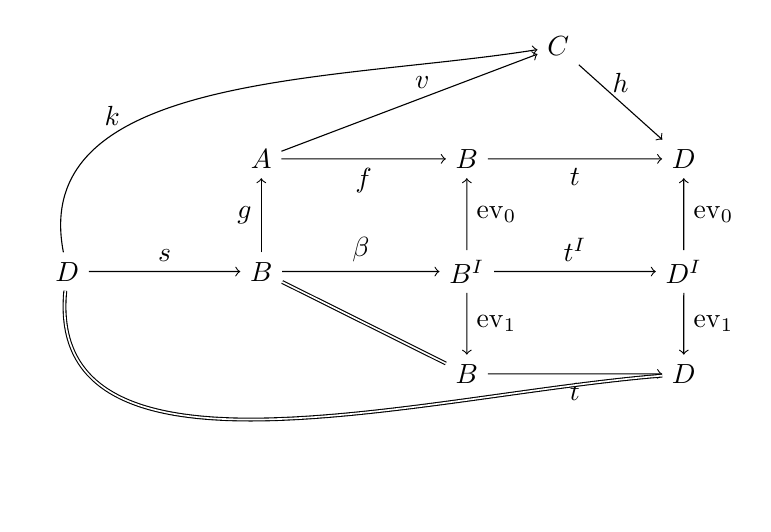
\begin{tikzpicture}[xscale=1.45,yscale=1.3]
\node (C) at (2.6,2.7) {$C$};
\node (A) at (0,1.6) {$A$};
\node (B) at (1.8,1.6) {$B$};
\node (D) at (3.7,1.6) {$D$};
\node (Dr) at (-1.7,0.5) {$D$};
\node (B3) at (0,0.5) {$B$};
\node (Bi) at (1.8,0.5) {$B^{\mathbb{I}}$};
\node (Di) at (3.7,0.5) {$D^{\mathbb{I}}$};
\node (Bb) at (1.8,-0.5) {$B$};
\node (Db) at (3.7,-0.5) {$D$};
\draw[->] (Dr) to[out=100,in=190] node[pos=0.3,above]{$k$} (C);
\draw[->] (A) -- (C) node[pos=0.55,above]{$v$};
\draw[->] (C) -- (D) node[midway,above]{$h$};
\draw[->] (A) -- (B) node[midway,below]{$f$};
\draw[->] (B) -- (D) node[midway,below]{$t$};
\draw[->] (B3) -- (A) node[midway,left]{$g$};
\draw[->] (Bi) -- (B) node[midway,right]{$\mathrm{ev}_0$};
\draw[->] (Di) -- (D) node[midway,right]{$\mathrm{ev}_0$};
\draw[->] (Dr) -- (B3) node[midway,above]{$s$};
\draw[->] (B3) -- (Bi) node[midway,above]{$\beta$};
\draw[->] (Bi) -- (Di) node[midway,above]{$t^{\mathbb{I}}$};
\draw[->] (Bi) -- (Bb) node[midway,right]{$\mathrm{ev}_1$};
\draw[->] (Di) -- (Db) node[midway,right]{$\mathrm{ev}_1$};
\draw[->] (Bb) -- (Db) node[midway,below]{$t$};
\draw[double] (B3) -- (Bb);
\draw[double] (Dr) to[out=-95,in=185] (Db);
\end{tikzpicture}
\end{center}
观察到 $v^{\mathbb{I}}\alpha u\colon C\to C^{\mathbb{I}}$
与 $t^{\mathbb{I}}\beta s\colon D\to D^{\mathbb{I}}$
定义了所需的\trHomotopyCoherentIsomorphism{}。

经由\cref{lem:equiv-homotopy-equivalences}，
\trEquivalence{}的\trTwoOfThreeProperty{}从%
\trQuasiCategory{}中\trIsomorphism{}之集对复合封闭这一事实推出。
\trQuasiCategory{}中的\trHomotopyCoherentIsomorphism{}表示\trHomotopyCategory{}中的\trIsomorphism{}，
其在\trHomotopyCategory{}中的复合是\trIsomorphism{}，
而由推论 1.1.16，
它可以被\trLifting{}为表示它的\trHomotopyCoherentIsomorphism{}。%
\footnote{事实上，由例 D.5.5，
\trHomotopyCoherentIsomorphism{}可以直接复合，但这里不需要这一点。}
现在我们把它用于\trInfinityCosmos{}的\trFunctorSpace{}中、
构成\trInfinityCategory{}之\trEquivalence{}数据一部分的
那些\trHomotopyCoherentIsomorphism{}。

要证\trEquivalence{}对复合封闭，
考虑一对可复合的\trEquivalence{}及其逆\trEquivalence
\begin{center}
\begin{tikzpicture}[xscale=1.7,yscale=1.1]
\node (A) at (0,0.6) {$A$};
\node (B) at (2,0.6) {$B$};
\node (C) at (4,0.6) {$C$};
\node (A2) at (0,-0.6) {$A$};
\node (B2) at (2,-0.6) {$B$};
\node (C2) at (4,-0.6) {$C$};
\draw[->] (A) -- (B) node[above]{$\overset{\simeq}{f}$};
\draw[->] (B) -- (C) node[above]{$\overset{\simeq}{g}$};
\draw[->] (B2) -- (A2) node[above]{$\overset{\simeq}{k}$};
\draw[->] (C2) -- (B2) node[above]{$\overset{\simeq}{h}$};
\end{tikzpicture}
\end{center}
\cref{lem:equiv-homotopy-equivalences} 的\trEquivalence{}数据定义\trIsomorphism
$\alpha\colon\mathrm{id}_A\cong kf\in\Fun(A,A)$
与 $\gamma\colon\mathrm{id}_B\cong hg\in\Fun(B,B)$，
后者经须状复合定义
$k\gamma f\colon kf\cong khgf\in\Fun(A,A)$。%
\yizhu{原书印作「$\Fun(B,B)$」，疑为「$\Fun(A,A)$」之误，此处径改。}
复合这两者，我们得到\trIsomorphism
$\mathrm{id}_A\cong khgf\in\Fun(A,A)$，
见证 $kh$ 定义 $gf$ 的左\trEquivalence{}逆。
另一\trIsomorphism{}类似地构造。

要证\trEquivalence{}对右消去封闭，考虑图表
\begin{center}
\begin{tikzpicture}[xscale=1.7,yscale=1.1]
\node (A) at (0,0) {$A$};
\node (B) at (2,0) {$B$};
\node (C) at (4,0) {$C$};
\draw[->] (C) to[out=140,in=40] node[above]{$\overset{\simeq}{\ell}$} (A);
\draw[->] (A) -- (B) node[above]{$\overset{\simeq}{f}$};
\draw[->] (B) -- (C) node[above]{$g$};
\draw[->] (B) -- (A) node[below]{$\overset{\simeq}{k}$};
\end{tikzpicture}
\end{center}
其中 $k$ 是 $f$ 的逆\trEquivalence{}，
而 $\ell$ 是 $gf$ 的逆\trEquivalence{}。
我们断言 $f\ell$ 定义 $g$ 的逆\trEquivalence{}。
所需的\trIsomorphism $\mathrm{id}_C\cong gf\ell$ 之一已经给出；
另一个通过复合 $\Fun(B,B)$ 中的三个\trIsomorphism{}得到
\begin{equation*}
\mathrm{id}_B
\xrightarrow[\ \beta^{-1}\ ]{\ \simeq\ }fk
\xrightarrow[\ f\delta k\ ]{\ \simeq\ }f\ell gfk
\xrightarrow[\ f\ell g\beta\ ]{\ \simeq\ }f\ell g.
\end{equation*}
\trEquivalence{}对左消去的稳定性之证明是对偶的。
\end{proof}

\trTrivialFibration{}容许一个类似的刻画，即作为\trSplitFiberHomotopyEquivalence{}。

\begin{lemma}[\trTrivialFibration{}分裂]\label{lem:trivial-fibrations-split}
每个\trTrivialFibration{}容许一个截面
\begin{center}
\begin{tikzpicture}[xscale=1.5,yscale=1.2]
\node (E) at (1.5,1.1) {$E$};
\node (BL) at (0,0) {$B$};
\node (BR) at (3,0) {$B$};
\draw[dashed,->] (BL) -- (E) node[pos=0.35,above,sloped]{$s$};
\draw[->] (E) -- (BR) node[midway,right]{$\overset{\simeq}{p}$};
\draw[double] (BL) -- (BR);
\end{tikzpicture}
\end{center}
该截面定义一个\trSplitFiberHomotopyEquivalence
\begin{center}
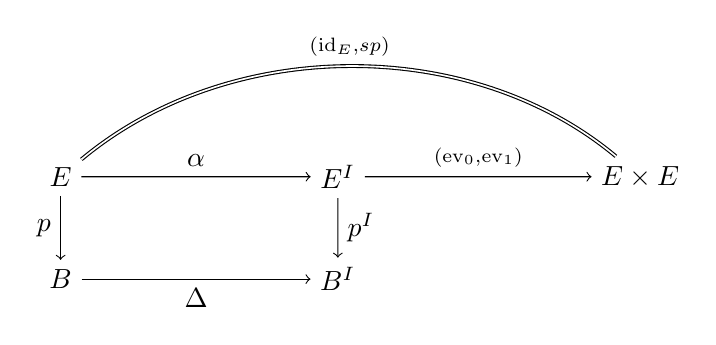
\begin{tikzpicture}[xscale=1.6,yscale=1.3]
\node (E) at (0,1) {$E$};
\node (Ei) at (2.2,1) {$E^{\mathbb{I}}$};
\node (EE) at (4.6,1) {$E\times E$};
\node (B) at (0,0) {$B$};
\node (Bi) at (2.2,0) {$B^{\mathbb{I}}$};
\draw[->] (E) -- (Ei) node[midway,above]{$\alpha$};
\draw[double] (E) to[out=45,in=135] node[midway,above]{$\scriptstyle(\mathrm{id}_E,sp)$} (EE);
\draw[->] (Ei) -- (EE) node[midway,above]{$\scriptstyle(\mathrm{ev}_0,\mathrm{ev}_1)$};
\draw[->] (E) -- (B) node[midway,left]{$p$};
\draw[->] (Ei) -- (Bi) node[midway,right]{$p^{\mathbb{I}}$};
\draw[->] (B) -- (Bi) node[midway,below]{$\Delta$};
\end{tikzpicture}
\end{center}
反之，任何定义\trSplitFiberHomotopyEquivalence{}的\trIsofibration{}%
是\trTrivialFibration{}。
\end{lemma}
\begin{proof}
若 $p\colon E\rvTfibArrow B$ 是\trTrivialFibration{}，
则由\cref{lem:trivial-fibration-stability}的末条稳定性性质，
对任意\trInfinityCategory{} $X$，
$p_\ast\colon\Fun(X,E)\rvTfibArrow\Fun(X,B)$ 亦然。
由定义 1.1.25，我们可以求解左下的\trLifting{}问题 %
\begin{equation*}
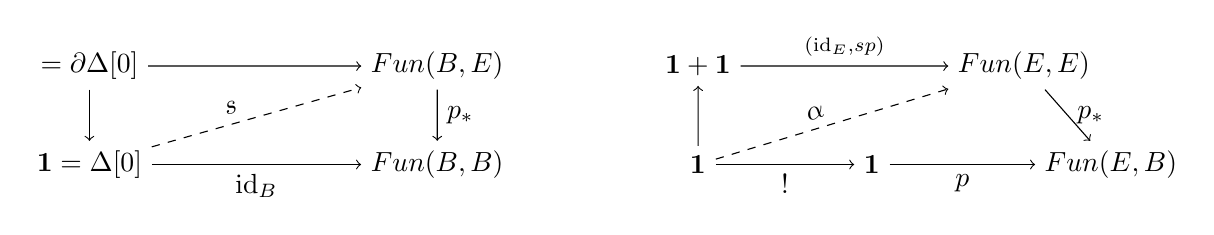
\begin{tikzpicture}[xscale=1.38,yscale=1.25]
\node (TL) at (0,1) {$\varnothing=\partial\Delta[0]$};
\node (TR) at (3.2,1) {$\Fun(B,E)$};
\node (BL) at (0,0) {$\mathbf{1}=\Delta[0]$};
\node (BR) at (3.2,0) {$\Fun(B,B)$};
\draw[->] (TL) -- (TR);
\draw[->] (TL) -- (BL);
\draw[->] (BL) -- (BR) node[midway,below]{$\mathrm{id}_B$};
\draw[->] (TR) -- (BR) node[midway,right]{$p_\ast$};
\draw[dashed,->] (BL) -- (TR) node[pos=0.4,above,sloped]{$s$};
\node at (4.5,0.5) {$\leftrightsquigarrow$};
\node (rTL) at (5.6,1) {$\mathbf{1}+\mathbf{1}$};
\node (rTR) at (8.6,1) {$\Fun(E,E)$};
\node (rBL) at (5.6,0) {$\mathbf{1}$};
\node (rBM) at (7.2,0) {$\mathbf{1}$};
\node (rBR) at (9.4,0) {$\Fun(E,B)$};
\draw[->] (rTL) -- (rTR) node[midway,above]{$\scriptstyle(\mathrm{id}_E,sp)$};
\draw[->] (rBL) -- (rTL);
\draw[->] (rBL) -- (rBM) node[midway,below]{$!$};
\draw[->] (rBM) -- (rBR) node[midway,below]{$p$};
\draw[->] (rTR) -- (rBR) node[midway,right]{$p_\ast$};
\draw[dashed,->] (rBL) -- (rTR) node[pos=0.45,above,sloped]{$\alpha$};
\end{tikzpicture}
\end{equation*}
求得映射 $s\colon B\to E$ 使得 $ps=\mathrm{id}_B$，
然后再求解右上的\trLifting{}问题，
以构造所需的\trFibration{}\trHomotopy{}。
逆命题由\cref{lem:equiv-homotopy-equivalences}立即得到。
\end{proof}

抽象\trHomotopy{}论中的一个经典构造证明了下面这条引理。

\begin{lemma}[Brown 分解引理]\label{lem:brown-factorization}
\trInfinityCosmos{}中的任何\trFunctor{} $f\colon A\to B$
都可以分解为一个\trEquivalence{}后接一个\trIsofibration{}，
其中该\trEquivalence{}被构造为某个\trTrivialFibration{}的截面。
\begin{rveq}\label{eq:brown-factorization}
\begin{tikzpicture}[xscale=1.5,yscale=1.2]
\node (Pf) at (0,1.3) {$Pf$};
\node (A) at (-2.2,0) {$A$};
\node (B) at (2.2,0) {$B$};
\draw[->] (A) -- (Pf) node[pos=0.55,above,sloped]{$\overset{\simeq}{q}$};
\draw[dashed,->] (-1.95,0.12) -- (-0.3,1.17) node[pos=0.35,below,sloped]{$s$};
\draw[->] (Pf) -- (B) node[pos=0.45,above,sloped]{$p$};
\draw[->] (A) -- (B) node[midway,below]{$f$};
\end{tikzpicture}
\end{rveq}
此外，$f$ 是\trEquivalence{}当且仅当%
\trIsofibration{} $p$ 是\trTrivialFibration{}。
\end{lemma}
\begin{proof}
图中所示的分解由一个\trIsofibration{}的\trPullback{}构造，
而该\trIsofibration{}由包含 $\mathbf{1}+\mathbf{1}\hookrightarrow\mathbb{I}$
到\trInfinityCategory{} $B$ 中的单纯\trCotensor{}形成。
\begin{center}
\begin{tikzpicture}[xscale=1.6,yscale=1.3]
\node (Ai) at (0,2) {$A^{\mathbb{I}}$};
\node (Bi) at (3,2) {$B^{\mathbb{I}}$};
\node (A) at (-2,1) {$A$};
\node (Pf) at (0.4,1) {$Pf$};
\node (AB) at (1.4,0) {$A\times B$};
\node (BB) at (3.6,0) {$B\times B$};
\draw[->] (A) -- (Ai) node[midway,above]{$\Delta$};
\draw[->] (Ai) -- (Bi) node[midway,above]{$f^{\mathbb{I}}$};
\draw[dashed,->] (A) -- (Pf) node[midway,above]{$\overset{\simeq}{s}$};
\draw[->] (Pf) -- (AB) node[midway,right]{$(q,p)$};
\draw[->] (A) -- (AB) node[pos=0.4,left]{$(A,f)$};
\draw[->] (AB) -- (BB) node[midway,below]{$f\times_B$};
\draw[->] (Bi) -- (BB) node[midway,right]{$\scriptstyle(\mathrm{ev}_0,\mathrm{ev}_1)$};
\node at (1.0,0.55) {$\scriptstyle\lrcorner$};
\end{tikzpicture}
\end{center}
注意映射 $q$ 是\trTrivialFibration
$\mathrm{ev}_0\colon B^{\mathbb{I}}\rvTfibArrow B$ 的\trPullback{}，
因而也是\trTrivialFibration{}。
它的截面 $s$ 通过把\trPullback{}的泛性质
用于所示的以 $A$ 为顶点的\trCone{}而构造，
于是由\trTwoOfThreeProperty{}它是\trEquivalence{}。
再由\trTwoOfThreeProperty{}，
$f$ 是\trEquivalence{}当且仅当 $p$ 是。
\end{proof}

\begin{remark}[\trEquivalence{}满足\trTwoOfSixProperty]\label{rem:equivalence-2-of-6}
事实上，任何\trInfinityCosmos{}中的\trEquivalence{}%
满足更强的\textbf{\trTwoOfSixProperty}（2-of-6 property）：
对任何可复合的\trFunctor{}三元组
\begin{center}
\begin{tikzpicture}[xscale=1.5,yscale=1.15]
\node (B) at (0,1.2) {$B$};
\node (A) at (-2.2,0) {$A$};
\node (D) at (2.2,0) {$D$};
\node (C) at (0,-1.2) {$C$};
\draw[->] (A) -- (B) node[pos=0.45,above,sloped]{$f$};
\draw[->] (B) -- (D) node[pos=0.45,above,sloped]{$\overset{\simeq}{hg}$};
\draw[->] (A) -- (D) node[pos=0.35,above]{$hgf$};
\draw[->] (B) -- (C) node[pos=0.68,right]{$g$};
\draw[->] (A) -- (C) node[pos=0.6,below,sloped]{$\overset{\simeq}{gf}$};
\draw[->] (C) -- (D) node[pos=0.5,below,sloped]{$h$};
\end{tikzpicture}
\end{center}
若 $gf$ 与 $hg$ 是\trEquivalence{}，
则 $f$、$g$、$h$ 与 $hgf$ 亦然。
Blumberg 与 Mandell 的一个论证 \cite[6.4]{bib20}
（在命题 C.1.8 中转述） %
利用 \cref{lem:equivalence-retracts-2-of-3}、\cref{lem:trivial-fibrations-split}
与 \cref{lem:brown-factorization}
证明\trEquivalence{}具有\trTwoOfSixProperty{}（见推论 C.1.9）。 %
\end{remark}

\trInfinityCosmos{}论进路之于抽象范畴论的一个关键优势在于：
从给定的\trInfinityCosmos{}出发，
可以构造出形形色色「\trFibration{}的」\trInfinityCosmos{}，
这意味着在这一公理框架中证明的任何定理
都可以特化并推广到那些情形。
这些导出的\trInfinityCosmos{}中最基本的，
是固定底对象之上的\trIsofibration{}的\trInfinityCosmos{}，
我们现在就引进它。
其他\trInfinityCosmos{}的例子将在第 6 章中发展，
那时我们对 \cref{def:infinity-cosmos}(i) 的宇宙论\trLimit{}会有更深入的理解。

\begin{proposition}[切片\trInfinityCosmos]\label{prop:sliced-cosmoi}
对任何\trInfinityCosmos{} $\mathcal{K}$
与任何\trInfinityCategory{} $B\in\mathcal{K}$，
存在一个由 $B$ 之上\trIsofibration{}组成的\trInfinityCosmos{} $\mathcal{K}_{/B}$，其
\begin{enumerate}[label=(\roman*)]
\item 对象是余域为 $B$ 的\trIsofibration{}
  $p\colon E\twoheadrightarrow B$
  \item \trFunctorSpace——比如说从 $p\colon E\twoheadrightarrow B$
  到 $q\colon F\twoheadrightarrow B$ 的——由\trPullback{}定义
\begin{center}
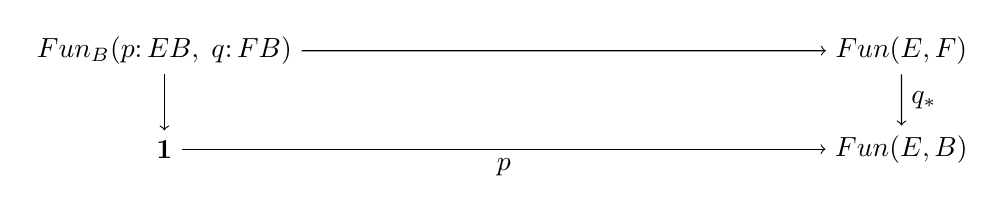
\begin{tikzpicture}[xscale=1.8,yscale=1.25]
\node (TL) at (0,1)
  {$\Fun_B(p\colon E\twoheadrightarrow B,\;q\colon F\twoheadrightarrow B)$};
\node (TR) at (5.2,1) {$\Fun(E,F)$};
\node (BL) at (0,0) {$\mathbf{1}$};
\node (BR) at (5.2,0) {$\Fun(E,B)$};
\draw[->] (TL) -- (TR);
\draw[->] (TL) -- (BL);
\draw[->] (TR) -- (BR) node[midway,right]{$q_\ast$};
\draw[->] (BL) -- (BR) node[midway,below]{$p$};
\node at (0.42,0.62) {$\scriptstyle\lrcorner$};
\end{tikzpicture}
\end{center}
且当指定的\trIsofibration{}在上下文中清楚时，
  缩记为 $\Fun_B(E,F)$
\item \trIsofibration{}是 $B$ 之上\trIsofibration{}的交换三角形
\begin{center}
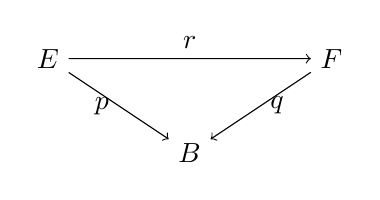
\begin{tikzpicture}[xscale=1.5,yscale=1.2]
\node (E) at (0,1) {$E$};
\node (F) at (2.4,1) {$F$};
\node (B) at (1.2,0) {$B$};
\draw[->] (E) -- (F) node[midway,above]{$r$};
\draw[->] (E) -- (B) node[pos=0.5,left]{$p$};
\draw[->] (F) -- (B) node[pos=0.5,right]{$q$};
\end{tikzpicture}
\end{center}
\item \trTerminal{}是 $\mathrm{id}\colon B\twoheadrightarrow B$，
  而积由沿对角的\trPullback{}定义
\begin{center}
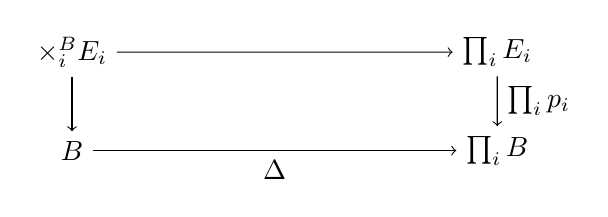
\begin{tikzpicture}[xscale=1.8,yscale=1.25]
\node (TL) at (0,1) {$\times_i^B E_i$};
\node (TR) at (3,1) {$\prod_i E_i$};
\node (BL) at (0,0) {$B$};
\node (BR) at (3,0) {$\prod_i B$};
\draw[->] (TL) -- (TR);
\draw[->] (TL) -- (BL);
\draw[->] (TR) -- (BR) node[midway,right]{$\prod_i p_i$};
\draw[->] (BL) -- (BR) node[midway,below]{$\Delta$};
\node at (0.42,0.62) {$\scriptstyle\lrcorner$};
\end{tikzpicture}
\end{center}
\item \trPullback{}与\trIsofibration{}之塔的\trLimit{}%
  由遗忘\trFunctor{} $\mathcal{K}_{/B}\to\mathcal{K}$ 造出
\item $p\colon E\twoheadrightarrow B$ 与 $U\in\sSet$
  的单纯\trCotensor{}由\trPullback{}构造
\begin{center}
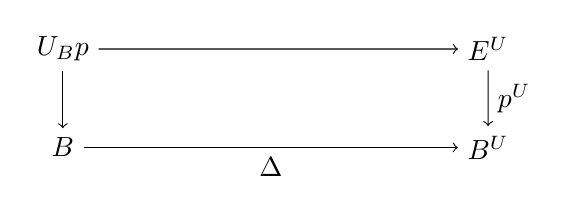
\begin{tikzpicture}[xscale=1.8,yscale=1.25]
\node (TL) at (0,1) {$U\pitchfork_B p$};
\node (TR) at (3,1) {$E^U$};
\node (BL) at (0,0) {$B$};
\node (BR) at (3,0) {$B^U$};
\draw[->] (TL) -- (TR);
\draw[->] (TL) -- (BL);
\draw[->] (TR) -- (BR) node[midway,right]{$p^U$};
\draw[->] (BL) -- (BR) node[midway,below]{$\Delta$};
\node at (0.42,0.62) {$\scriptstyle\lrcorner$};
\end{tikzpicture}
\end{center}
\item 并且其中 $B$ 之上的映射
\begin{center}
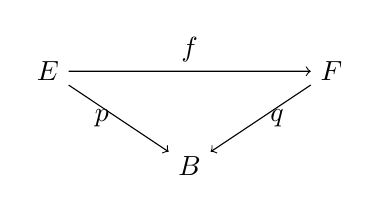
\begin{tikzpicture}[xscale=1.5,yscale=1.2]
\node (E) at (0,1) {$E$};
\node (F) at (2.4,1) {$F$};
\node (B) at (1.2,0) {$B$};
\draw[->] (E) -- (F) node[midway,above]{$f$};
\draw[->] (E) -- (B) node[pos=0.5,left]{$p$};
\draw[->] (F) -- (B) node[pos=0.5,right]{$q$};
\end{tikzpicture}
\end{center}
是\trInfinityCosmos{} $\mathcal{K}_{/B}$ 中的\trEquivalence{}，
  当且仅当 $f$ 是 $\mathcal{K}$ 中的\trEquivalence{}。
\end{enumerate}
\end{proposition}
\begin{proof}
\trFunctorSpace{}是\trQuasiCategory{}，
因为 \cref{def:infinity-cosmos}(ii) 断言：
对 $\mathcal{K}$ 中任何\trIsofibration{} $q\colon F\twoheadrightarrow B$，
映射 $q_\ast\colon\Fun(E,F)\twoheadrightarrow\Fun(E,B)$
是\trQuasiCategory{}的\trIsofibration{}。
该公理的其他部分蕴含：
每个\trLimit{}构造——如在 (iv) 与 (vi) 中构造的积与\trCotensor——
都定义 $B$ 之上的\trIsofibration{}。
$\mathcal{K}_{/B}$ 中\trIsofibration{}的诸封闭性质
从 $\mathcal{K}$ 中相应的封闭性质推出。
其中最复杂的是 $\mathcal{K}_{/B}$ 中\trIsofibration{}的
Leibniz \trCotensor{}稳定性，
它从 $\mathcal{K}$ 中相应的性质推出：
因为对\trSimplicialSet{}的\trMonomorphism $i\colon X\hookrightarrow Y$
与如上面 (iii) 中 $B$ 之上的\trIsofibration{} $r$，
映射 $i\widehat{\pitchfork}_B r$
由沿 $\Delta\colon B\to B^Y$ \trPullback $i\widehat{\pitchfork} r$ 而构造。

上述构造在一个单纯富集切片\trCategory{}中
定义单纯富集\trLimit{}这一事实，
是富集范畴论的标准结果。

只剩下验证\trIsofibration{}的\trInfinityCosmos{}中的%
\trEquivalence{}由遗忘\trFunctor{} $\mathcal{K}_{/B}\to\mathcal{K}$ 造出。
先设 (vii) 中所示的映射 $f$ 定义 $\mathcal{K}$ 中的\trEquivalence{}。
那么对任何\trIsofibration{} $s\colon A\twoheadrightarrow B$，
$\mathcal{K}_{/B}$ 中\trFunctorSpace{}上诱导的映射由\trPullback{}定义
\begin{equation*}
\begin{tikzpicture}[xscale=1.75,yscale=1.3]
\node (TL) at (0,2) {$\Fun_B(A,E)$};
\node (TR) at (4,2) {$\Fun(A,E)$};
\node (ML) at (1.7,1) {$\Fun_B(A,F)$};
\node (MR) at (5.6,1) {$\Fun(A,F)$};
\node (BL) at (0,0) {$\mathbf{1}$};
\node (BR) at (4,0) {$\Fun(A,B)$};
\draw[->] (TL) -- (TR) node[midway,above]{$f_\ast$};
\draw[->] (TL) -- (BL);
\draw[dashed,->] (TL) -- (ML) node[pos=0.5,above,sloped]{$\overset{\simeq}{f_\ast}$};
\draw[->] (ML) -- (MR) node[midway,above]{$p_\ast$};
\draw[->] (ML) -- (BL);
\draw[->] (TR) -- (MR) node[pos=0.45,above,sloped]{$\overset{\simeq}{f_\ast}$};
\draw[->] (TR) -- (BR) node[midway,right]{$p_\ast$};
\draw[->] (MR) -- (BR) node[pos=0.45,right]{$q_\ast$};
\draw[->] (BL) -- (BR) node[midway,below]{$s$};
\node at (0.42,1.62) {$\scriptstyle\lrcorner$};
\node at (2.12,0.62) {$\scriptstyle\lrcorner$};
\end{tikzpicture}
\end{equation*}
由于 $f$ 是 $\mathcal{K}$ 中的\trEquivalence{}，
映射 $f_\ast\colon\Fun(A,E)\to\Fun(A,F)$ 是\trEquivalence{}，
于是在 $s$ 之上的纤维上诱导的映射也是\trEquivalence{}。%
\footnote{\trIsofibration{}之间的\trEquivalence{}在\trPullback{}下的稳定性，
既可以作为\cref{lem:trivial-fibration-stability}与 \cref{lem:brown-factorization}的推论、
用单纯\trHomotopy{}论的标准技术来证明（见引理 C.1.11），
也可以按 2-\trCategory{}的方式论证（见命题 3.3.4）。}

对于逆蕴涵，我们求助于\cref{lem:equiv-homotopy-equivalences}。
若 $f\colon E\to F$ 是 $\mathcal{K}_{/B}$ 中的\trEquivalence{}，
则它在 $\mathcal{K}_{/B}$ 中容许\trHomotopy{}逆。
逆\trEquivalence{} $g\colon F\to E$ 也定义 $\mathcal{K}$ 中的逆\trEquivalence{}，
而 $\mathcal{K}$ 中所需的单纯\trHomotopy
\begin{equation*}
E\xrightarrow{\ \alpha\ }\mathbb{I}\pitchfork_B p\longrightarrow E^{\mathbb{I}}
\qquad\qquad
F\xrightarrow{\ \beta\ }\mathbb{I}\pitchfork_B q\longrightarrow F^{\mathbb{I}}
\end{equation*}
通过沿定义 $\mathcal{K}_{/B}$ 中\trCotensor{}的\trPullback{}之顶边作复合而定义。
\end{proof}

如\cref{dig:source-cosmoi-nature}中所提到的，
我们遇到的许多「野外」\trInfinityCosmos{}%
满足一条附加公理。
然而注意，这条公理不被\cref{prop:sliced-cosmoi}的切片\trInfinityCosmos{}继承，
这是它未被纳入\cref{def:infinity-cosmos}的原因之一。

\begin{definition}[\trCartesianClosed\trInfinityCosmos]\label{def:cartesian-closed-cosmoi}
一个\trInfinityCosmos{} $\mathcal{K}$ 是\textbf{\trCartesianClosed}
（cartesian closed），
如果积双\trFunctor{} $-\times-\colon\mathcal{K}\times\mathcal{K}\to\mathcal{K}$
扩充为一个单纯富集的双变量\trAdjunction
\begin{equation*}
\Fun(A\times B,C)\cong\Fun(A,C^B)\cong\Fun(B,C^A)
\end{equation*}
其中右\trAdjunction{} $(-)^A\colon\mathcal{K}\to\mathcal{K}$
对一切 $A\in\mathcal{K}$ 保持\trIsofibration{}。
\end{definition}
例如，\trQuasiCategory{}的\trInfinityCosmos{}是\trCartesianClosed{}，
其指数被定义为单纯\trCotensor{}的（特例）。
这正是我们对\trCotensor{}与指数使用同一记号的原因之一。
\footnote{这一方便的记号混用的其他优点
在 2.3 节与命题 10.3.5 中讨论。}

注意此时\trFunctorSpace{}与指数相重合。
\trCategory{}与\trKanComplex{}的笛卡尔封闭\trInfinityCosmos{}也是如此。
一般地，从 $A$ 到 $B$ 的\trFunctorSpace
是指数 $B^A$ 的「底\trQuasiCategory」——只要后者存在（见注 1.3.11）。

\begin{example}[$(\infty,1)$-\trCategory{}的\trInfinityCosmos{}；附录 E.2]\label{exa:cosmoi-models}
下列 $(\infty,1)$-\trCategory{}的模型定义\trCartesianClosed\trInfinityCosmos{}：
\begin{enumerate}[label=(\roman*)]
  \item Rezk 的\textbf{\trCompleteSegalSpaces}（complete Segal spaces）
  定义一个\trInfinityCosmos{} $\CSS$ 的对象，
  其中\trIsofibration{}、\trEquivalence{}与\trTrivialFibration
  是文献 \cite{bib100} 的\trModelStructure{}的相应类。%
  \footnote{警告：\trCompleteSegalSpaces{}的\trModelCategory
  在两个不同的「方向」上富集于\trSimplicialSet——
  一种富集使两个\trCompleteSegalSpaces{}之间的映射\trSimplicialSet
  成为\trKanComplex{}，探测「空间的」结构；
  另一种富集使映射\trSimplicialSet{}成为\trQuasiCategory{}，
  探测「\trCategory{}的」结构 \cite{bib64}。
  我们要的是后一种富集。}
\item 由 Dwyer、Kan 与 Smith \cite{bib38} 定义、
  并由 Hirschowitz 与 Simpson \cite{bib56} 发展的
  \textbf{\trSegalCategories}（Segal categories）
  定义一个\trInfinityCosmos{} $\mathcal{S}egal$ 的对象，
  其中\trIsofibration{}、\trEquivalence{}与\trTrivialFibration
  是文献 \cite{bib13,bib90} 的\trModelStructure{}的相应类。%
  \footnote{这里我们把术语「\trSegalCategories{}」保留给
  那些带有离散对象集、Reedy \trFibration{}且满足 Segal 条件的单纯对象。
  传统定义不包含 Reedy \trFibration{}条件，
  因为由\trKanComplex\trEnrichedCategory{}的\trNerve{}定义的单纯对象不满足它。
  由于\trKanComplex\trEnrichedCategory
  不在我们偏好的 $(\infty,1)$-\trCategory{}模型之列，
  这一点并不困扰我们。}
\item 文献 \cite{bib129} 的\textbf{\trOneComplicialSets}（1-complicial sets），
  \trEquivalence{}地，文献 \cite{bib78} 的「自然带标记\trQuasiCategory」，
  定义一个\trInfinityCosmos{} $1\text{-}\mathcal{C}omp$ 的对象，
  其中\trIsofibration{}、\trEquivalence{}与\trTrivialFibration
  是这两个来源中任一者的\trModelStructure{}的相应类。
\end{enumerate}
\end{example}

在附录 E.3 中，我们将证明
$(\infty,n)$-\trCategory{}乃至 $(\infty,\infty)$-\trCategory{}的某些模型
定义\trInfinityCosmos{}：
$n$-\trQuasiCategory{}、$\Theta_n$-空间、
迭代\trCompleteSegalSpaces{}以及 $n$-复状单纯集。

\begin{definition}[\trCodualInfinityCosmos]\label{def:co-dual-cosmoi}
存在一个对象上恒等的对合\trFunctor{}
$(-)^\circ\colon\boldsymbol{\Delta}\to\boldsymbol{\Delta}$，
它反转每个序数 $[n]\in\boldsymbol{\Delta}$ 中元素的顺序。
在 1.1.1 的记号下，\trFunctor $(-)^\circ$
把面映射 $\delta^i\colon[n-1]\rightarrowtail[n]$
送到面映射 $\delta^{n-i}\colon[n-1]\rightarrowtail[n]$，
并把退化映射 $\sigma^i\colon[n+1]\twoheadrightarrow[n]$
送到退化映射 $\sigma^{n-i}\colon[n+1]\twoheadrightarrow[n]$。
与这一对合自\trIsomorphism{}作\trPreComposition{}诱导一个对合
$(-)^{op}\colon\sSet\to\sSet$，
它把\trSimplicialSet $X$ 送到其\textbf{\trOppositeSimplicialSet}
（opposite simplicial set）$X^{op}$，
每个单纯形中顶点的定向被反转。
这一构造保持所有\trCone{}形\trLimit{}与\trColimit{}，
并在指数上诱导\trIsomorphism
$(Y^X)^{op}\cong(Y^{op})^{X^{op}}$。
\end{definition}

对任何\trInfinityCosmos{} $\mathcal{K}$，
存在一个\textbf{\trDualInfinityCosmos}
（dual ∞-cosmos）$\mathcal{K}^{co}$：
对象与 $\mathcal{K}$ 相同，但\trFunctorSpace{}定义为 %
\begin{equation*}
\Fun_{\mathcal{K}^{co}}(A,B):=\Fun_{\mathcal{K}}(A,B)^{op}.
\end{equation*}
$\mathcal{K}^{co}$ 中的\trIsofibration{}、\trEquivalence{}%
与\trTrivialFibration
与 $\mathcal{K}$ 中的相重合。

$\mathcal{K}^{co}$ 中的\trCone{}形\trLimit{}与 $\mathcal{K}$ 中的相重合，
而 $A\in\mathcal{K}$ 与 $U\in\sSet$ 的\trCotensor %
则定义为 $A^{U^{op}}$。

这一记号的一个 2-范畴论辩护见练习 1.4.ii。

\begin{definition}[离散\trInfinityCategory]\label{def:discrete-infinity-categories}
\trInfinityCosmos{} $\mathcal{K}$ 中的\trInfinityCategory{} $E$
是\textbf{\trDiscrete}（discrete），
如果对一切 $X\in\mathcal{K}$，
\trFunctorSpace $\Fun(X,E)$ 是\trKanComplex{}。
\end{definition}
在\trQuasiCategory{}的\trInfinityCosmos{}中，
离散\trInfinityCategory{}恰是\trKanComplex{}。
类似地，在\cref{exa:cosmoi-models}的那些\trInfinityCosmos{}中——
其\trInfinityCategory{}是某种模型下的 $(\infty,1)$-\trCategory——
离散\trInfinityCategory{}是\trInfinityGroupoid{}。
对下文重要的是，
离散\trInfinityCategory{}可以在\trInfinityCosmos{}之内
如下「内在地」刻画：

\begin{lemma}\label{lem:discrete-trivial-fibration}
\trInfinityCategory{} $E$ 是\trDiscrete{}，当且仅当
$E^{\mathbb{I}}\rvTfibArrow E^{\mathbf{2}}$ 是\trTrivialFibration{}。
\end{lemma}
\begin{proof}
由\cref{def:equivalence-trivial-fibration}，
\trIsofibration $E^{\mathbb{I}}\twoheadrightarrow E^{\mathbf{2}}$
是\trTrivialFibration{}，当且仅当对一切\trInfinityCategory{} $X$，
\trFunctorSpace{}上诱导的映射 %
\begin{equation*}
\begin{array}{ccc}
\Fun(X,E^{\mathbb{I}}) & \longrightarrow & \Fun(X,E^{\mathbf{2}})\\[0.4ex]
{\scriptstyle\cong}\downarrow & & \downarrow{\scriptstyle\cong}\\[0.4ex]
\Fun(X,E)^{\mathbb{I}} & \longrightarrow & \Fun(X,E)^{\mathbf{2}}
\end{array}
\end{equation*}
是\trQuasiCategory{}的\trTrivialFibration{}。
经由单纯\trCotensor{}的泛性质，
引理 1.1.30 告诉我们：
该映射是\trTrivialFibration{}，当且仅当 $\Fun(X,E)$ 是\trKanComplex{}。
\end{proof}
读者可以验证：
任何\trInfinityCosmos{}中的离散\trInfinityCategory{}%
装配成一个\trInfinityCosmos{} $\mathcal{K}^{\simeq}$。
证明见命题 6.1.6，
那里发展了从给定者产生新的\trInfinityCosmos{}的一般技术。

\subsection*{练习}

\begin{exercise}\label{ex:simplicial-versus-enriched}
在下列二\trCategory{}之间定义\trEquivalence{}：
\begin{enumerate}[label=(\roman*)]
  \item \trSimplicialCategory{}，如 \eqref{eq:simplicial-category-diagram} 中者，与
\item 富集于\trSimplicialSet{}的\trCategory{}。
\end{enumerate}
\end{exercise}

\begin{exercise}\label{ex:conical-products-qcat}
详细展开\cref{prop:cosmos-quasi-categories}的证明：
证明\trSimpliciallyEnrichedCategory $\QCat$
容许满足\cref{dig:simplicially-enriched-limits}之泛性质的\trCone{}形积。即：
\begin{enumerate}[label=(\roman*)]
\item 定义一对\trQuasiCategory $A$ 与 $B$ 的笛卡尔积 $A\times B$
  及投影映射 $\pi_A\colon A\times B\to A$
  与 $\pi_B\colon A\times B\to B$，
  并证明这组数据满足通常的（非富集的）泛性质。
\item 给定另一个\trQuasiCategory $X$，
  用 (i) 与\trYonedaLemma{}证明投影映射诱导\trQuasiCategory{}的\trIsomorphism
  \begin{equation*}
  (A\times B)^X\xrightarrow{\ \simeq\ }A^X\times B^X.
  \end{equation*}
\item 解释这与\cref{dig:simplicially-enriched-limits}的泛性质有何关系。
\item 把 (i) 的通常 1-范畴论泛性质
  表述为 (ii) 之泛性质的「$0$ 维面向」。
\end{enumerate}
\end{exercise}

\begin{exercise}\label{ex:path-object}
证明\trInfinityCosmos{}中的任何对象都有\textbf{\trPathObject}
（path object）
\begin{center}
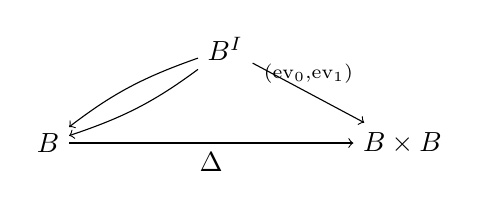
\begin{tikzpicture}[xscale=1.5,yscale=1.2]
\node (Bi) at (1.5,1) {$B^{\mathbb{I}}$};
\node (B) at (0,0) {$B$};
\node (BB) at (3,0) {$B\times B$};
\draw[->] (Bi) to[bend right=10] (B);
\draw[->] (Bi) to[bend left=10] (B);
\draw[->] (Bi) -- (BB) node[midway,above]{$\scriptstyle(\mathrm{ev}_0,\mathrm{ev}_1)$};
\draw[->] (B) -- (BB) node[midway,below]{$\Delta$};
\end{tikzpicture}
\end{center}
它由与\trFreeLivingIsomorphism{}作\trCotensor{}而构造。
\end{exercise}

\begin{exercise}\label{ex:dual-cartesian-closed}
证明：若 $\mathcal{K}$ 是\trCartesianClosed\trInfinityCosmos{}，
则 $\mathcal{K}^{co}$ 亦然。
\end{exercise}

\begin{exercise}[6.1.6]\label{ex:discrete-cosmos}
用\cref{prop:cosmos-kan-complexes}证明：
任何\trInfinityCosmos{}中的离散\trInfinityCategory{}%
定义一个\trInfinityCosmos{}，
其\trFunctorSpace{}皆为\trKanComplex{}。
\end{exercise}
